%\packagelist
\documentclass[10pt]{article}
\usepackage[top=3cm, bottom=3cm, outer=3cm, inner=3cm]{geometry}
\usepackage{multicol}
\usepackage{graphicx}
\usepackage{url}
%\usepackage{cite}
\usepackage{hyperref}
\usepackage{array}
%\usepackage{multicol}
\newcolumntype{x}[1]{>{\centering\arraybackslash\hspace{0pt}}p{#1}}
\usepackage{natbib}
\usepackage{pdfpages}
\usepackage{multirow}
\usepackage[normalem]{ulem}

\useunder{\uline}{\ul}{}
\usepackage{svg}
\usepackage{xcolor}
\usepackage{listings}

\lstdefinestyle{ascii-tree}{
    literate={├}{|}1 {─}{--}1 {└}{+}1 
  }
\lstset{basicstyle=\ttfamily,
  showstringspaces=false,
  commentstyle=\color{red},
  keywordstyle=\color{blue}
}
%\usepackage{booktabs}
\usepackage{caption}
\usepackage{subcaption}
\usepackage{float}
\usepackage{array}

\newcolumntype{M}[1]{>{\centering\arraybackslash}m{#1}}
\newcolumntype{N}{@{}m{0pt}@{}}


%%%%%%%%%%%%%%%%%%%%%%%%%%%%%%%%%%%%%%%%%%%%%%%%%%%%%%%%%%%%%%%%%%%%%%%%%%%%
%%%%%%%%%%%%%%%%%%%%%%%%%%%%%%%%%%%%%%%%%%%%%%%%%%%%%%%%%%%%%%%%%%%%%%%%%%%%
\newcommand{\itemEmail}{rchambillap@unsa.edu.pe}
\newcommand{\itemStudent}{Chambilla Perca Ricardo Mauricio}
\newcommand{\itemCourse}{Programacion Web 2}
\newcommand{\itemCourseCode}{1701213}
\newcommand{\itemSemester}{III}
\newcommand{\itemUniversity}{Universidad Nacional de San Agustín de Arequipa}
\newcommand{\itemFaculty}{Facultad de Ingeniería de Producción y Servicios}
\newcommand{\itemDepartment}{Departamento Académico de Ingeniería de Sistemas e Informática}
\newcommand{\itemSchool}{Escuela Profesional de Ingeniería de Sistemas}
\newcommand{\itemAcademic}{2024 - A}
\newcommand{\itemInput}{Del 8 de Mayo 2024}
\newcommand{\itemOutput}{Al 15 de Mayo 2024}
\newcommand{\itemPracticeNumber}{1}
\newcommand{\itemTheme}{GitHub}
%%%%%%%%%%%%%%%%%%%%%%%%%%%%%%%%%%%%%%%%%%%%%%%%%%%%%%%%%%%%%%%%%%%%%%%%%%%%
%%%%%%%%%%%%%%%%%%%%%%%%%%%%%%%%%%%%%%%%%%%%%%%%%%%%%%%%%%%%%%%%%%%%%%%%%%%%

\usepackage[english,spanish]{babel}
\usepackage[utf8]{inputenc}
\AtBeginDocument{\selectlanguage{spanish}}
\renewcommand{\figurename}{Figura}
\renewcommand{\refname}{Referencias}
\renewcommand{\tablename}{Tabla} %esto no funciona cuando se usa babel
\AtBeginDocument{%
	\renewcommand\tablename{Tabla}
}

\usepackage{fancyhdr}
\pagestyle{fancy}
\fancyhf{}
\setlength{\headheight}{30pt}
\renewcommand{\headrulewidth}{1pt}
\renewcommand{\footrulewidth}{1pt}
\fancyhead[L]{\raisebox{-0.2\height}{
\includegraphics[width=3cm]{./img/logo_episunsa.png}}}
\fancyhead[C]{\fontsize{7}{7}\selectfont	\itemUniversity \\ \itemFaculty \\ \itemDepartment \\ \itemSchool \\ \textbf{\itemCourse}}
\fancyhead[R]{\raisebox{-0.2\height}{
\includegraphics[width=1.2cm]{./img/logo_abet}}}
\fancyfoot[L]{Estudiante Ricardo Ch}
\fancyfoot[C]{\itemCourse}
\fancyfoot[R]{Página \thepage}

% para el codigo fuente 
\usepackage{listings}
\usepackage{color, colortbl}
\definecolor{numberOrange}{RGB}{235, 126, 9}
\definecolor{mygreen}{RGB}{40, 194, 6}
\definecolor{dkgreen}{rgb}{0,0.6,0}
\definecolor{myblue}{RGB}{57, 118, 189}
\definecolor{gray}{rgb}{0.156,0.146,0.135}
\definecolor{mygray}{RGB}{135, 135, 135}
\definecolor{mauve}{rgb}{0.58,0,0.82}
\definecolor{codebackgroundCode}{RGB}{10, 10, 20}
\definecolor{codebackgroundBash}{rgb}{0.95, 0.95, 0.92}
\definecolor{tablebackground}{rgb}{0.8, 0, 0}


\lstdefinestyle{java}{frame=tb,
	language=Java,
	showstringspaces=false,
	columns=flexible,
	basicstyle={\footnotesize\ttfamily\color[RGB]{255,255,255}},
	numberstyle=\color{mygray},
	numbers=left, 
	keywordstyle=\color{myblue},
	morekeywords={String, System},
	commentstyle=\color{mygray},
	stringstyle=\color{mygreen},
	breaklines=true,
	breakatwhitespace=true,
	tabsize=2,
	backgroundcolor= \color{codebackgroundCode},
	showspaces=false,
	showtabs=false,
	showlines=false,
}

\lstdefinestyle{mybash}{frame=tb,
	language=bash,
	showstringspaces=false,
	columns=flexible,
	keepspaces=true,
	basicstyle={\small\ttfamily},
	numberstyle=\color{mygray},
	keywordstyle=\color{myblue},
	morekeywords={java, javac},
	commentstyle=\color{mygray},
	stringstyle=\color{mygreen},
	breaklines=true,
	breakatwhitespace=true,
	tabsize=2,
	backgroundcolor= \color{codebackgroundBash},
	showspaces=false,
	showtabs=false,
	showlines=false,
}

\begin{document}
\lstset{
    literate={─}{--}2 {├}{|---}2 {└}{|---}2
}
	\vspace*{10px}
	
	\begin{center}	
		\fontsize{17}{17} \textbf{ Informe de Laboratorio 2}
	\end{center}
	\centerline{\textbf{\Large Tema: \itemTheme}}
	%\vspace*{0.5cm}	

	\begin{flushright}
		\begin{tabular}{|M{2.5cm}|N|}
			\hline
			\rowcolor{tablebackground}
			\color{white} \textbf{Nota}  \\
			\hline 
			     \\[30pt]
			\hline 			
		\end{tabular}
	\end{flushright}	

	\begin{table}[H]
		\begin{tabular}{|x{4.7cm}|x{4.8cm}|x{4.8cm}|}
			\hline 
			\rowcolor{tablebackground}
			\color{white} \textbf{Estudiante} & \color{white}\textbf{Escuela}  & \color{white}\textbf{Asignatura}   \\
			\hline 
			{\itemStudent \par \itemEmail} & \itemSchool & {\itemCourse \par Semestre: \itemSemester \par Código: \itemCourseCode}     \\
			\hline 			
		\end{tabular}
	\end{table}		
	
	\begin{table}[H]
		\begin{tabular}{|x{4.7cm}|x{4.8cm}|x{4.8cm}|}
			\hline 
			\rowcolor{tablebackground}
			\color{white}\textbf{Laboratorio} & \color{white}\textbf{Tema}  & \color{white}\textbf{Duración}   \\
			\hline 
			\itemPracticeNumber & \itemTheme & 08  \\
			\hline 
		\end{tabular}
	\end{table}
	
	\begin{table}[H]
		\begin{tabular}{|x{4.7cm}|x{4.8cm}|x{4.8cm}|}
			\hline 
			\rowcolor{tablebackground}
			\color{white}\textbf{Semestre académico} & \color{white}\textbf{Fecha de inicio}  & \color{white}\textbf{Fecha de entrega}   \\
			\hline 
			\itemAcademic & \itemInput &  \itemOutput  \\
			\hline 
		\end{tabular}
	\end{table}
	
	
	\section{DESCRIPCION DE ACTIVIDAD}
	\subsection{Elabore un informe individual, de estudio de Git y GitHub. \newline
	Cree su página personal con las recomendaciones dadas por la W3C en su tutorial de CSS: Em-
	pezando con HTML y CSS: https://www.w3.org/Style/Examples/011/firstcss.en.html.
	}
	
	Estoy usando como base una pagina html que presentamos antes en pweb1.\newline
	La cual se ve así: \newline

	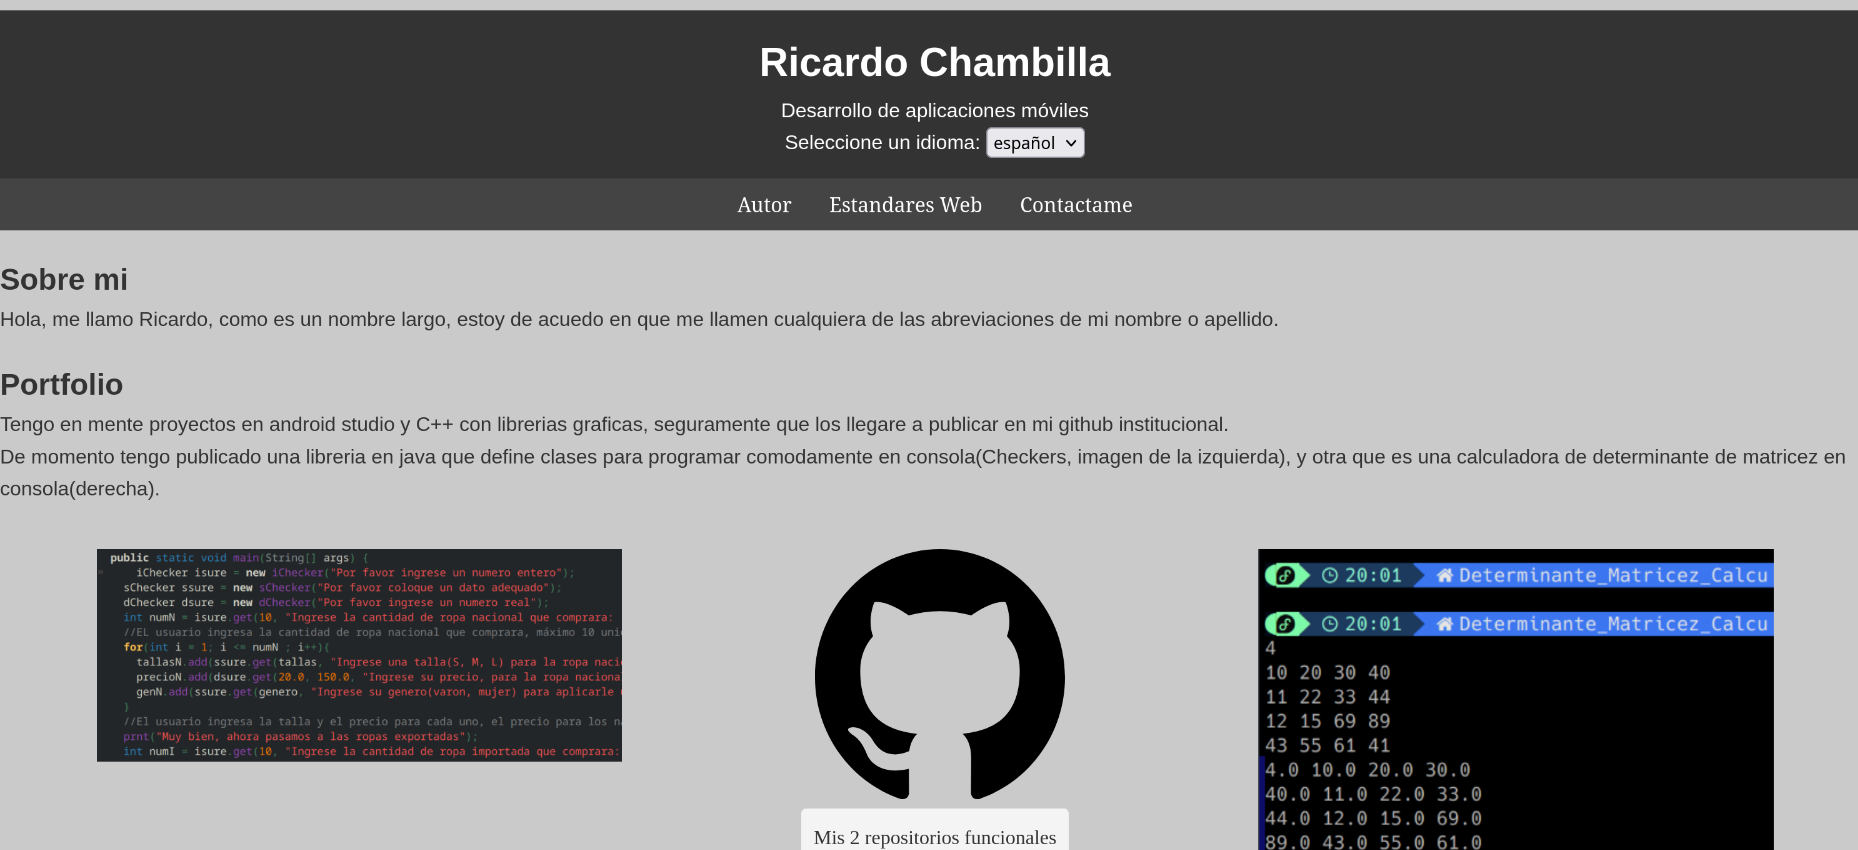
\includegraphics[scale=0.25]{./img/lab2_1.png}


	\subsection{Requerimientos}
	index.html - (Menú principal - Página principal de bienvenida al sitio beb)
	autor.html - (Menú principal - Página de presentación del autor) (Se activa Menú Izquierdo)
	hobbies.html - (Menú Izquierdo - Página de fotos y descripciones de sus hobbies.)
	hngSoftware.html - (Menú Izquierdo - Página donde explique ¿Qué es la Ing. de Software desde su punto de vista?. Descripción, especialidades que resalte.)
	haleria.html - (Menú Izquierdo - Página de fotos y descripciones libres que quiera compartir.)
	estandaresWeb.html- (Menú principal - Página donde describa la W3C y algunos estándares web.)
contactame.html- (Menú principal - Página donde muestra un formulario de contacto.)\newline
Menú Principal |*Inicio|Autor|Estándares Web|Contáctame|\newline
Inicio: Página de presentación del sitio. "Bienvenido a ...".\newline
Autor: Descripción del autor. "Mi nombre es ...".\newline
Estándares Web: SVG, WOFF, WebRTC, XML.\newline
Contáctame: Formulario: |nombres:input| |correo:email| |genero:radiobutton| |nacimiento:date| |asunto:input| |contenido:textarea| |enviar:button|\newline
Menú Izquierdo |*Autor| ->|Hobbies|Ing. de Software|Galería| \newline
Hobbies: Descripción, tiempo, recomendaciones, fotos. \newline
Ing. de Software: Acerca de la carrera de Ing. de Software. Futuro. Especialidad. \newline
Contactanos: Formulario que guarda en una base de datos. Las consutas que se desean enviar: nombres, correo electrónico, asunto, detalle..\newline
Utilice todas las recomendaciones dadas por el docente: \newline

	\section{Pregunta}
	
	\subsection{Mencione tres aportes a su adquisición de conocimientos que este laboratorio le proporcionó.}
	
	El primero seria que ahora conocemos nuestro primer software de regulador de versiones (git)\newline
	El segundo conocimiento que me llevo de esta clase es que existen buenas practicas y estandares en el desarrollo web.\newline
	El tercero el flujo de trabajo de git, y por su extension github.

\pagebreak

	\section{\textcolor{red}{Rúbricas}}
	
	\subsection{\textcolor{red}{Entregable Informe}}
	\begin{table}[H]
		\caption{Tipo de Informe}
		\setlength{\tabcolsep}{0.5em} % for the horizontal padding
		{\renewcommand{\arraystretch}{1.5}% for the vertical padding
		\begin{tabular}{|p{3cm}|p{12cm}|}
			\hline
			\multicolumn{2}{|c|}{\textbf{\textcolor{red}{Informe}}}  \\
			\hline 
			\textbf{\textcolor{red}{Latex}} & \textcolor{blue}{El informe está en formato PDF desde Latex,  con un formato limpio (buena presentación) y facil de leer.}   \\ 
			\hline 
			
			
		\end{tabular}
	}
	\end{table}
	
	\subsection{\textcolor{red}{Rúbrica para el contenido del Informe y demostración}}
	\begin{itemize}			
		\item El alumno debe marcar o dejar en blanco en celdas de la columna \textbf{Checklist} si cumplio con el ítem correspondiente.
		\item Si un alumno supera la fecha de entrega,  su calificación será sobre la nota mínima aprobada, siempre y cuando cumpla con todos lo items.
		\item El alumno debe autocalificarse en la columna \textbf{Estudiante} de acuerdo a la siguiente tabla:
	
		\begin{table}[ht]
			\caption{Niveles de desempeño}
			\begin{center}
			\begin{tabular}{ccccc}
    			\hline
    			 & \multicolumn{4}{c}{Nivel}\\
    			\cline{1-5}
    			\textbf{Puntos} & Insatisfactorio 25\%& En Proceso 50\% & Satisfactorio 75\% & Sobresaliente 100\%\\
    			\textbf{2.0}&0.5&1.0&1.5&2.0\\
    			\textbf{4.0}&1.0&2.0&3.0&4.0\\
    		\hline
			\end{tabular}
		\end{center}
	\end{table}	
	
	\end{itemize}
	
	\begin{table}[H]
		\caption{Rúbrica para contenido del Informe y demostración}
		\setlength{\tabcolsep}{0.5em} % for the horizontal padding
		{\renewcommand{\arraystretch}{1.5}% for the vertical padding
		%\begin{center}
		\begin{tabular}{|p{2.7cm}|p{7cm}|x{1.3cm}|p{1.2cm}|p{1.5cm}|p{1.1cm}|}
			\hline
    		\multicolumn{2}{|c|}{Contenido y demostración} & Puntos & Checklist & Estudiante & Profesor\\
			\hline
			\textbf{1. GitHub} & Hay enlace URL activo del directorio para el  laboratorio hacia su repositorio GitHub con código fuente terminado y fácil de revisar. &2 &X &1 & \\ 
			\hline
			\textbf{2. Commits} &  Hay capturas de pantalla de los commits más importantes con sus explicaciones detalladas. (El profesor puede preguntar para refrendar calificación). &4 &X &0 & \\ 
			\hline 
			\textbf{3. Código fuente} &  Hay porciones de código fuente importantes con numeración y explicaciones detalladas de sus funciones. &2 &X &1 & \\ 
			\hline 
			\textbf{4. Ejecución} & Se incluyen ejecuciones/pruebas del código fuente  explicadas gradualmente. &2 &X &1 & \\ 
			\hline			
			\textbf{5. Pregunta} & Se responde con completitud a la pregunta formulada en la tarea.  (El profesor puede preguntar para refrendar calificación).  &2 &X &1 & \\ 
			\hline	
			\textbf{6. Fechas} & Las fechas de modificación del código fuente estan dentro de los plazos de fecha de entrega establecidos. &2 &X &0 & \\ 
			\hline 
			\textbf{7. Ortografía} & El documento no muestra errores ortográficos. &2 &X &2 & \\ 
			\hline 
			\textbf{8. Madurez} & El Informe muestra de manera general una evolución de la madurez del código fuente,  explicaciones puntuales pero precisas.  &4 &X &2 & \\ 
			\hline
			\multicolumn{2}{|c|}{\textbf{Total}} &20 & &08 & \\ 
			\hline
		\end{tabular}
		%\end{center}
		%\label{tab:multicol}
		}
	\end{table}
	
\clearpage

\section{Referencias}
\begin{itemize}			
	\item \url{https://drive.google.com/file/d/19hjCsMtViypEj3cOPRF_cflH1r8r9vBn/view?usp=sharing}
\end{itemize}	
	
%\clearpage
%\bibliographystyle{apalike}
%\bibliographystyle{IEEEtranN}
%\bibliography{bibliography}
			
\end{document}